% (If you have SVG figures, convert them to PDF/PNG for best compatibility.)
% =====================================================================
%  Blog post template: compiles in Overleaf AND builds on the website.
%
%  Overleaf:  New Project -> Upload Project -> overleaf-post.zip
%             (main document = index.tex, compiler = pdfLaTeX)
%  Publish:   Overleaf Menu -> Download -> Source (.zip), unzip into
%             posts/<yyyy-mm-short-name>/ in the blog repo, edit meta.yaml,
%             then git add / commit / push.
%
%  Rules that keep both outputs working:
%   * Title, date, category, summary live in meta.yaml (not \title/abstract;
%     the website ignores those).
%   * Figures: PNG/JPG/PDF in figs/, referenced as figs/<name>.
%   * Define macros with \providecommand (the site also defines them).
%   * Number equations with \label{eq:...} and cite them with \eqref{...}.
% =====================================================================
\documentclass[11pt]{article}
\usepackage[margin=2.5cm]{geometry}
\usepackage{amsmath, amssymb}
\usepackage{graphicx}
\usepackage[round]{natbib} % enables \citet / \citep
\usepackage{listings}
\usepackage{xcolor}
\usepackage{hyperref}
\usepackage{booktabs} 
\usepackage{tabularx}
\usepackage[table]{xcolor}
\usepackage{pgfplots}

\lstset{basicstyle=\ttfamily\small, columns=fullflexible, frame=single, breaklines=true}

\definecolor{okfg}{HTML}{1F7A4D}
\definecolor{nearfg}{HTML}{8A6A00}
\definecolor{missfg}{HTML}{B3322B}
\definecolor{statedbg}{HTML}{DBE9F7}
\definecolor{tickbg}{HTML}{EFE3FA}
\definecolor{sftcol}{HTML}{2F6FB3}
\definecolor{grpocol}{HTML}{B4561F}
\newcommand{\errok}[1]{\textcolor{okfg}{\textbf{#1}}}
\newcommand{\errnear}[1]{\textcolor{nearfg}{\textbf{#1}}}
\newcommand{\errmiss}[1]{\textcolor{missfg}{\textbf{#1}}}
\setlength{\fboxsep}{1pt}
\newcommand{\stated}[1]{\colorbox{statedbg}{\strut #1}}
\newcommand{\tick}[1]{\colorbox{tickbg}{\strut #1}}

% Shared site macros (same as macros.tex in the blog repo)
\providecommand{\dd}{\mathrm{d}}
\providecommand{\dv}[2]{\frac{\mathrm{d}#1}{\mathrm{d}#2}}
\providecommand{\pdv}[2]{\frac{\partial #1}{\partial #2}}
\providecommand{\tr}{\operatorname{tr}}

% Shown only in the PDF; the website uses meta.yaml
\title{Teaching a VLM to Read Analog Clocks: SFT and GRPO}
\author{Sodtavilan Odonchimed}
\date{}

\begin{document}
\maketitle


I found this research~\citep{choi2026itstimerightimproving} about VLMs on analog clock recognition. The results are shown in the paper; VLMs accuracies are not good at clock recognition. In this note, I trained the recent local VLM models using SFT and GRPO.

The study discusses why it is challenging for VLMs; datasets of this kind have the following things:
\begin{enumerate}
    \item \textbf{Spatial recognition:} Clocks appear at random positions in the image, and in some cases only part of the clock is visible.
    \item \textbf{Clock design:} Clocks vary widely. Some have no numerals, while others use Roman numerals.
\end{enumerate}
The authors also built TickTockVQA, a dataset for clock recognition. It contains:
\begin{itemize}
    \item Training images: 7,236
    \item Evaluation images: 5,247
\end{itemize}
The images were collected from OpenImages, COCO, ClockMovies, VisualGenome, CC12M, ImageNet, and SBU.


\section{SFT}
First, I ran SFT training~\citep{pareja2024unveilingsecretrecipeguide}. I sampled 765 images (7,236 was too many) from the training set. Following the paper, I also generated 5000 synthetic clock images, for a total of 5,765 training images.
The SFT hyperparameters were as follows:
\begin{table}[h]
\centering
\begin{tabular}{ll}
\hline
\textbf{Hyperparameter} & \textbf{Value} \\
\hline
LoRA $r$ & 64 \\
LoRA $\alpha$ & 128 \\
LoRA dropout & 0.05 \\
Training steps & 360 \\
\hline
\end{tabular}
\end{table}
To recap LoRA $r$ and $\alpha$ ~\citep{hu2021loralowrankadaptationlarge}: let $W$ be a weight matrix of the pretrained VLM. The part that LoRA updates is $\Delta W$, which can be factorized as $\Delta W = BA$. If $W \in \mathbb{R}^{D \times D}$, then $B \in \mathbb{R}^{D \times r}$ and $A \in \mathbb{R}^{r \times D}$. LoRA $r$ is the dimension of the compressed representation. The final weight is:
$$W' = W + \frac{\alpha}{r}BA.$$
And LoRA $\alpha$ acts as a scaling factor. Here are the training curves of the SFT. 

\begin{figure}[t]
  \centering
  \begin{minipage}{0.49\linewidth}
    \centering
    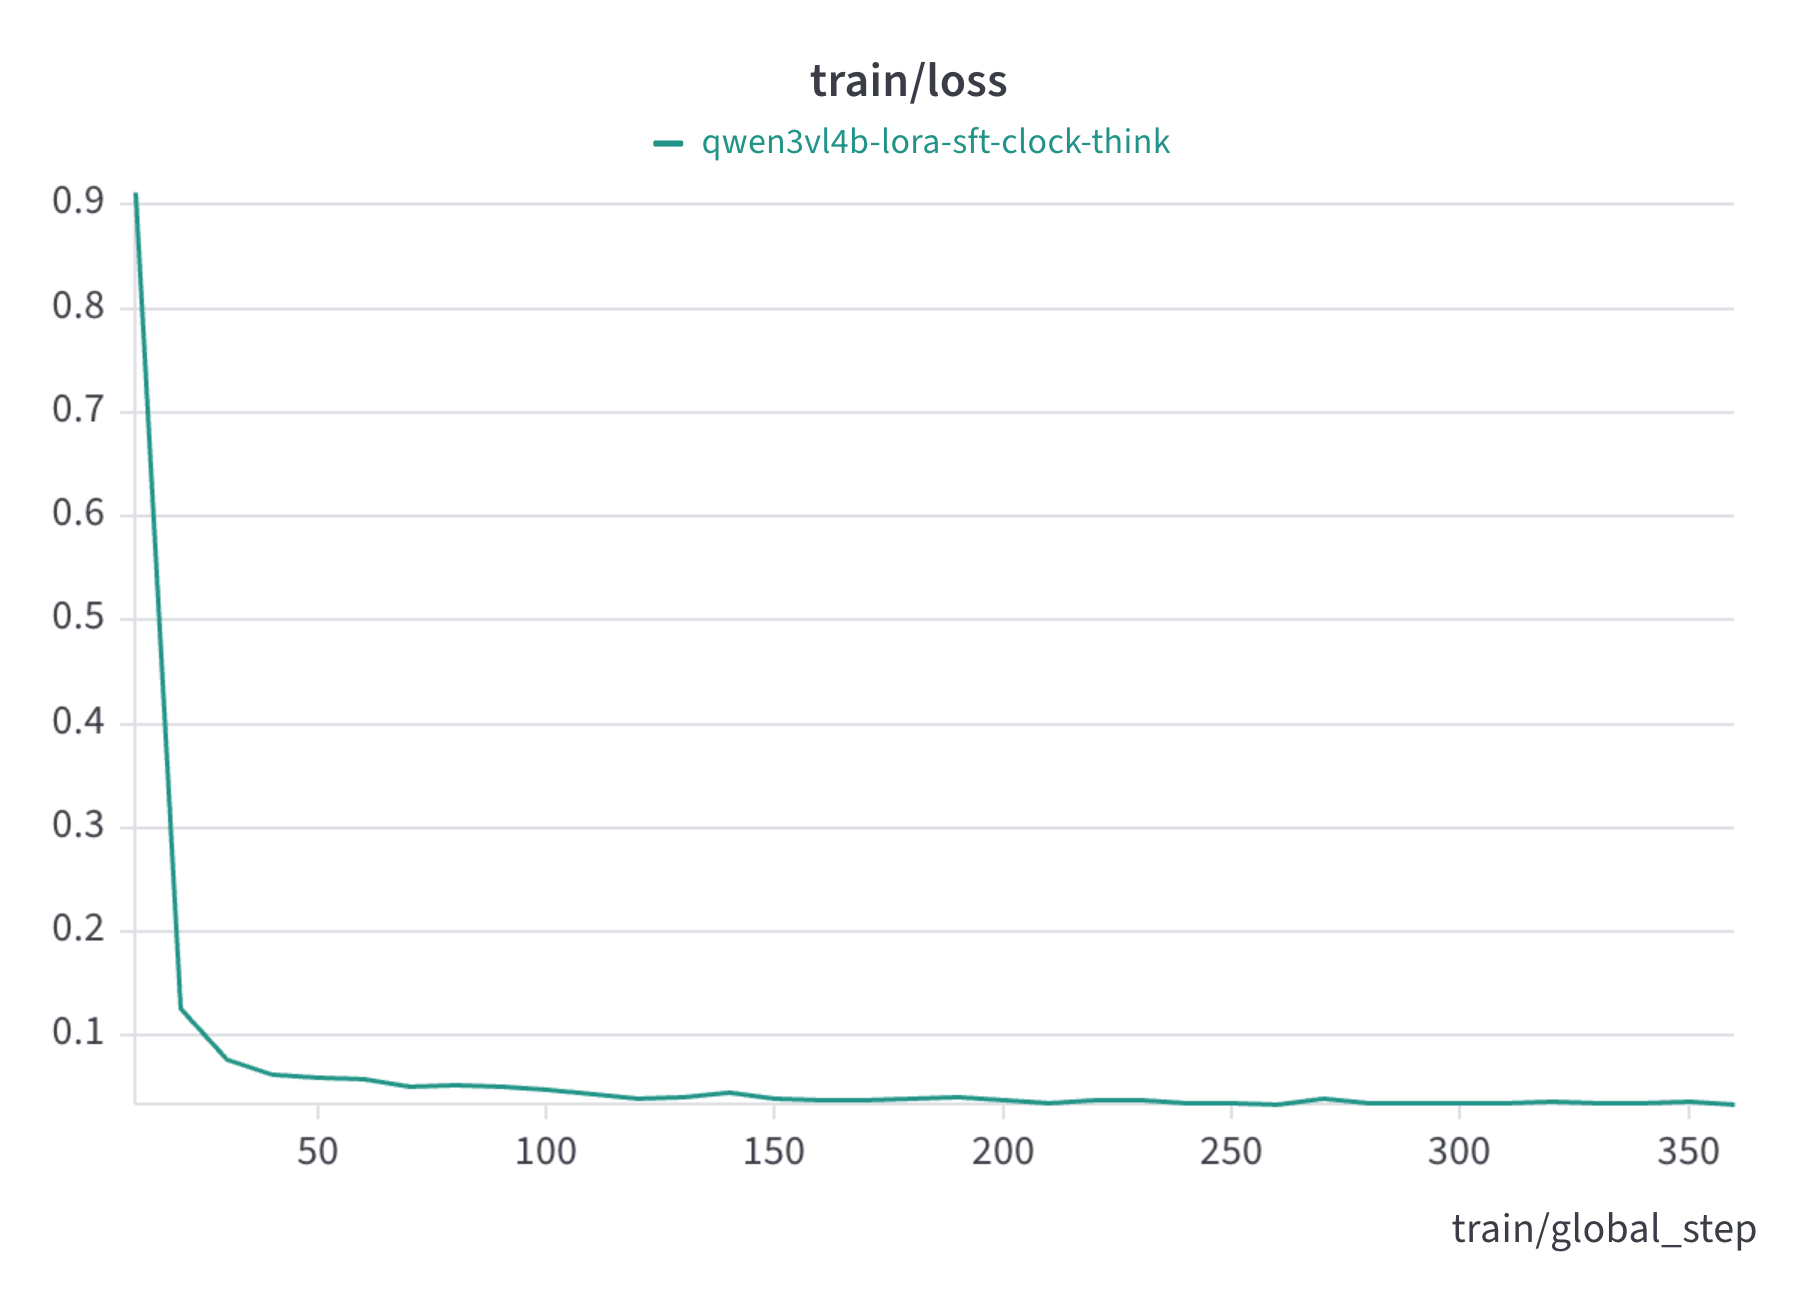
\includegraphics[width=\linewidth]{figs/clock-vlm-loss.png}
    \small\textbf{Loss}
  \end{minipage}\hfill
  \begin{minipage}{0.49\linewidth}
    \centering
    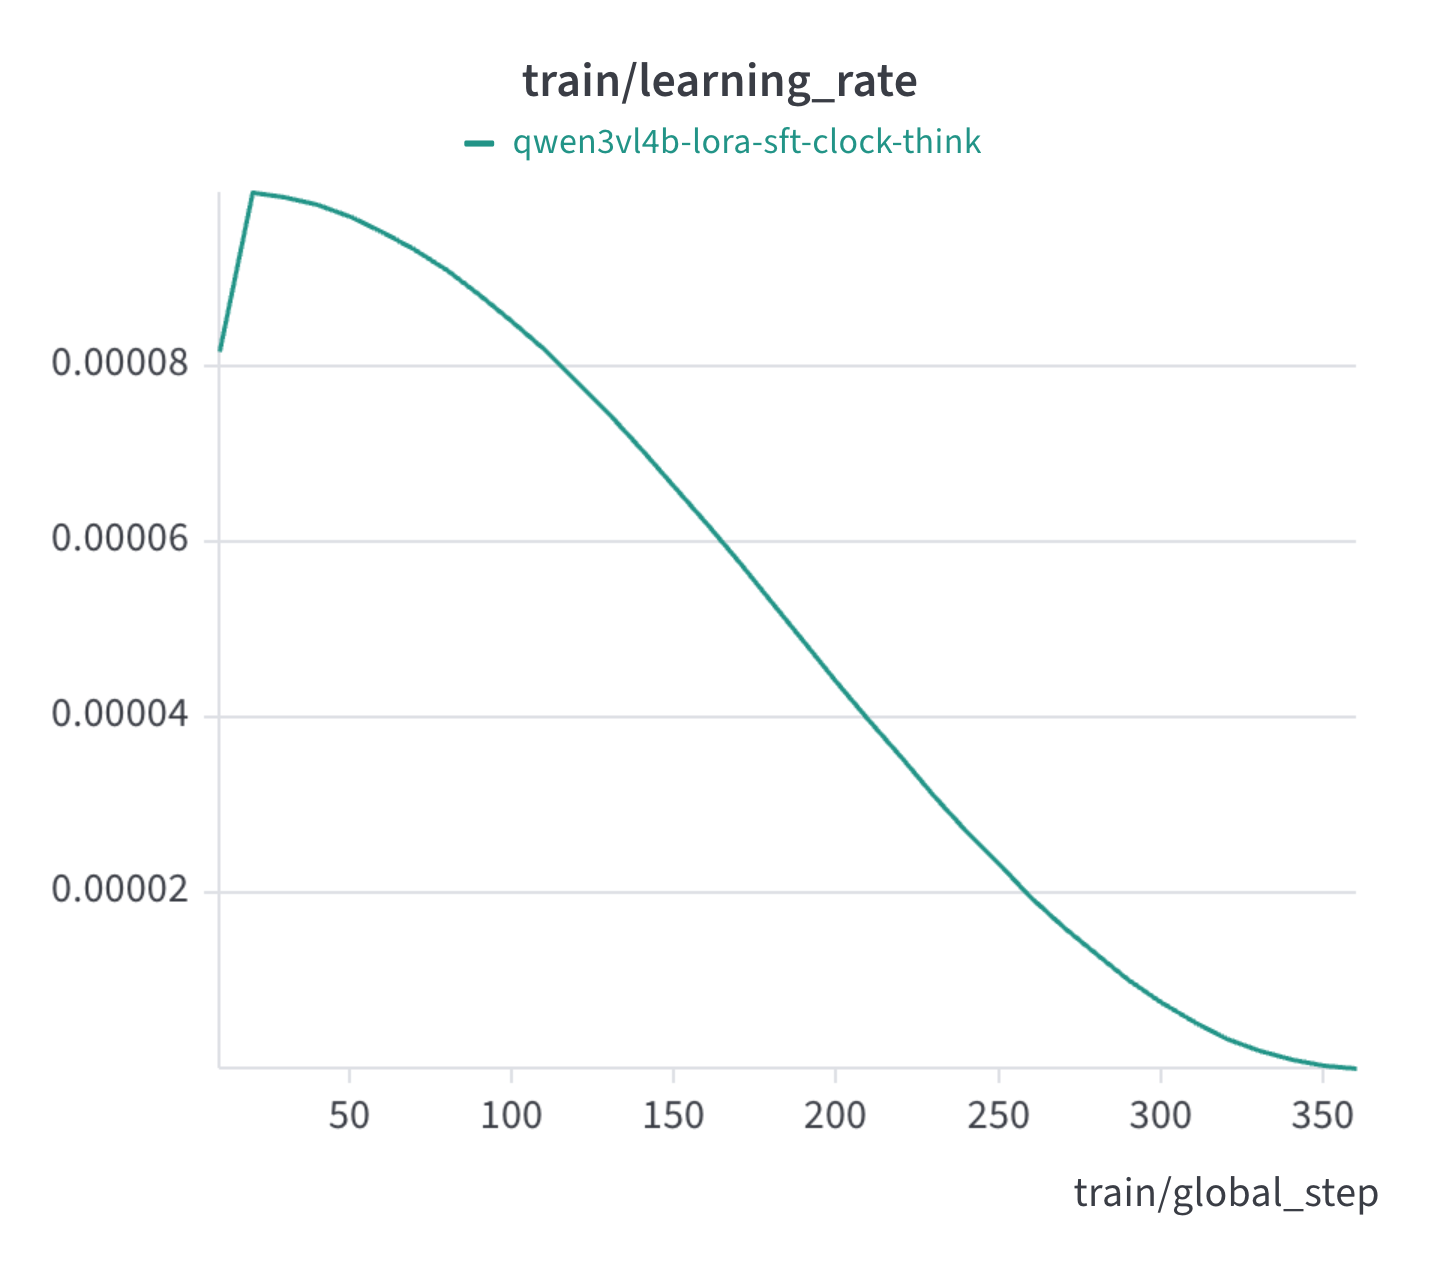
\includegraphics[width=\linewidth]{figs/clock-vlm-lr.png}
    \small\textbf{Learning rate}
  \end{minipage}
  \caption{SFT training curves.}
  \label{fig:sft-training-curves}
\end{figure}

\section{GRPO}
Next, I tried Group Relative Policy Optimization (GRPO)~\citep{shao2024deepseekmathpushinglimitsmathematical}, the method used in DeepSeek-R1, to see whether it could improve performance further. GRPO is a RL method that uses two types of reward: a format reward, which encourages the model to output the correct format (e.g., <thinking> tags), and an accuracy reward, which checks whether the answer is correct.

And, GRPO involves the following three policies:
\begin{itemize}
    \item $\pi_\mathrm{old}$: the policy at the time the samples (outputs $o_i$) were generated
    \item $\pi_\mathrm{ref}$: a fixed model that serves as the reference for KL regularization; usually the SFT model from before reinforcement learning
    \item $\pi_\theta$: the policy model being trained (the only one that is updated)
\end{itemize}
Let $q$ be the input question. To compute the objective function $J$, we generate $N$ samples and take their average:

$$J(\theta) = \mathbb{E}_{\{o_i\}_i ^N \sim \pi_\mathrm{old}}\left[\frac{1}{N}\sum_{i=1}^N\left\{ \min(s_1 \cdot A_i, s_2 \cdot A_i) - \beta D_{KL}[\pi_\theta || \pi_\mathrm{ref}] \right\} \right].$$

Here, $s_1=\frac{\pi_\theta (o_i|q)}{\pi_\mathrm{old}(o_i|q)}$, $s_2=\mathrm{clip}(s_1, 1-\epsilon, 1+\epsilon)$, and $A_i=\frac{r_i - \mathrm{mean}(r_1, r_2, ..., r_N)}{\mathrm{std}(r_1, r_2, ..., r_N)}$. We compute the gradients that maximize the objective function $J$.

In this work, I implemented the following reward functions:
\begin{itemize}
    \item \textbf{robust time reward:} Since time is a continuous quantity, I designed a robust reward function.
    \item \textbf{consistency reward:} Rewards the LLM for outputting answers in the format "The time is H:MM".
    \item \textbf{format reward:} Rewards the <thinking> tags and the correct output format.
\end{itemize}
The training data was the same as for SFT, and the training steps are 200.
\begin{figure}[htbp]
  \centering
  \begin{minipage}{0.49\linewidth}
    \centering
    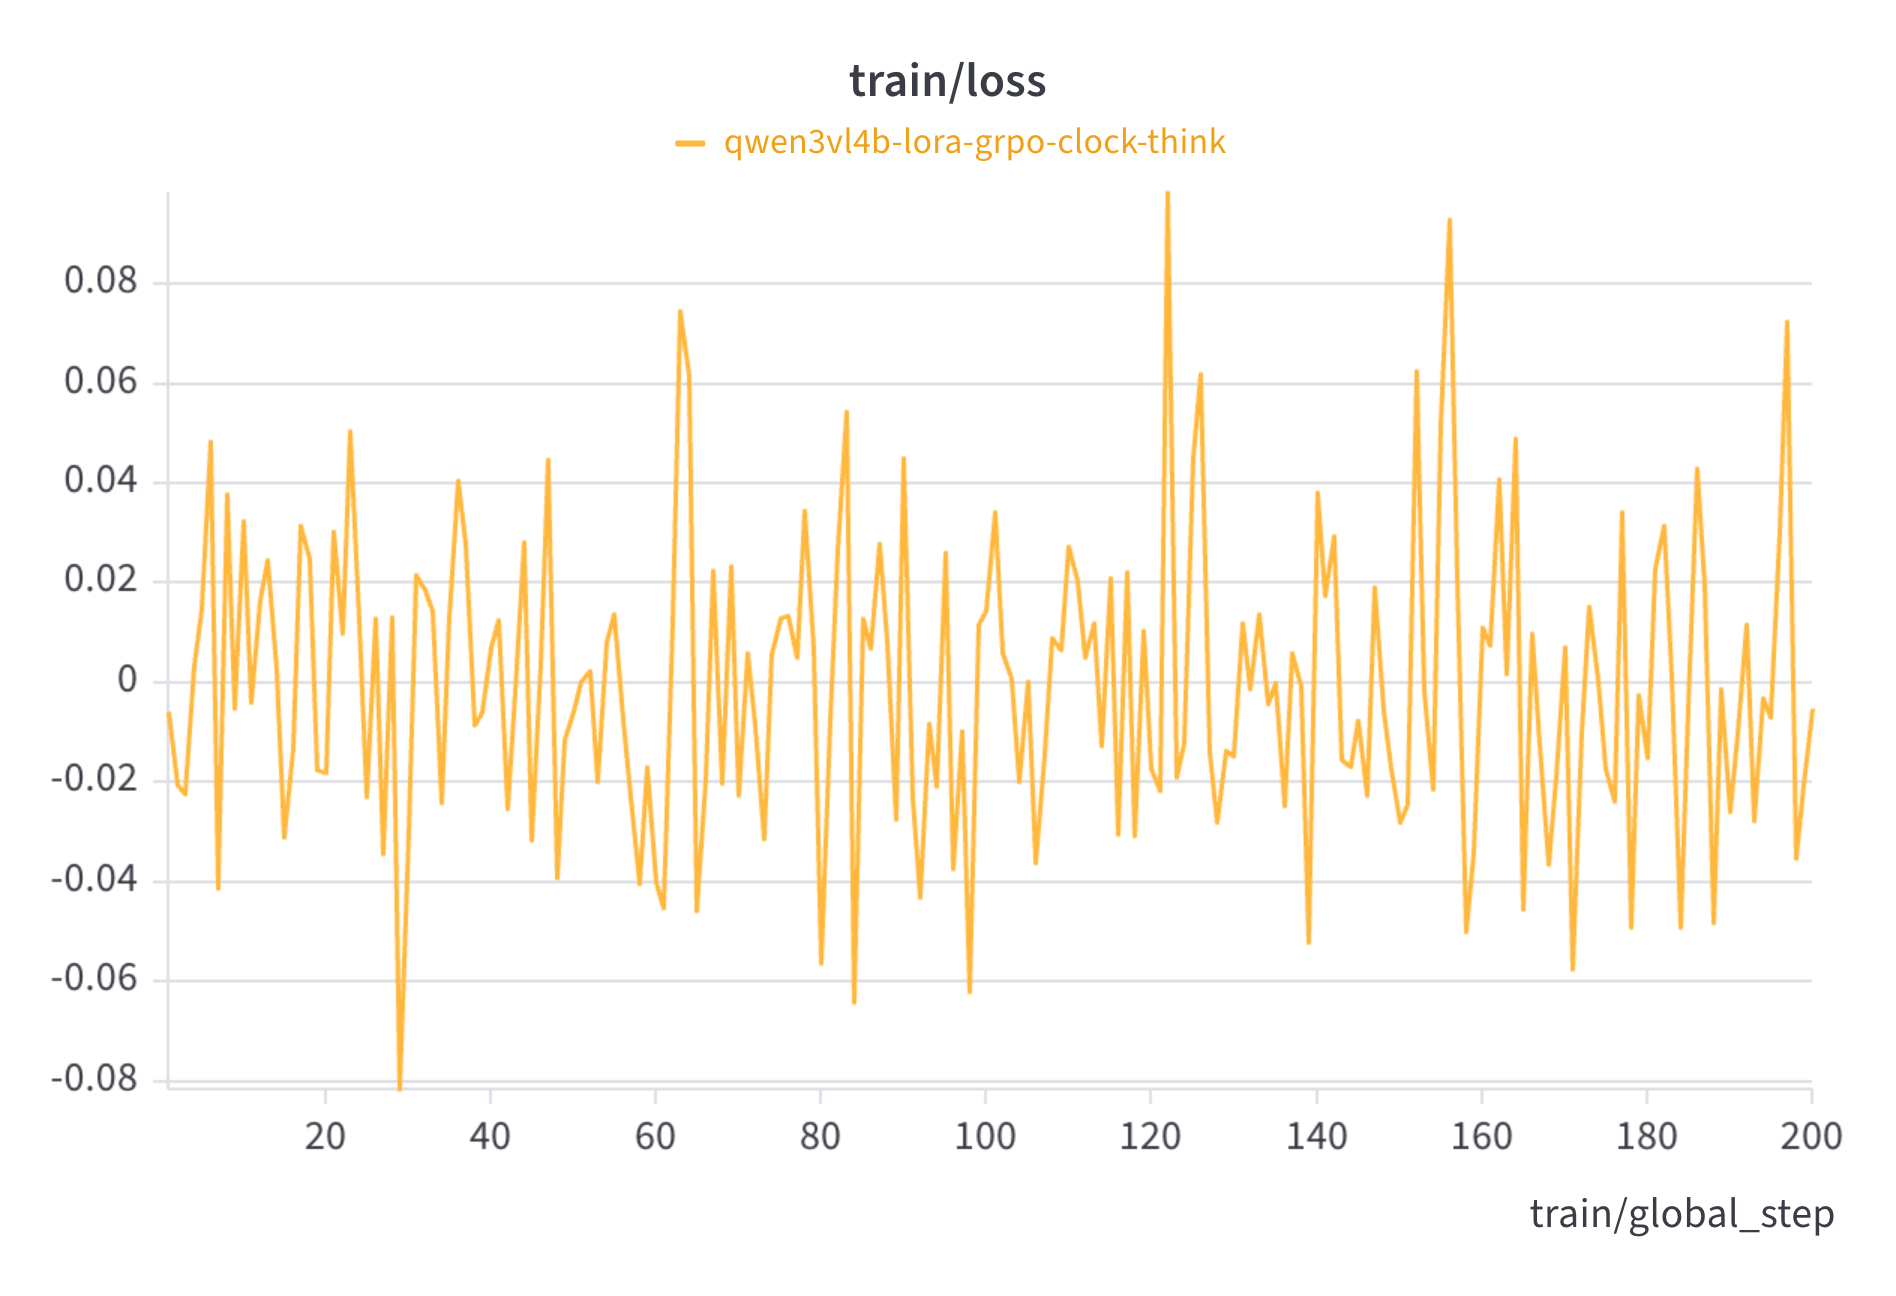
\includegraphics[width=\linewidth]{figs/clock-vlm-grpo-loss.png}
    \small\textbf{Loss}
  \end{minipage}\hfill
  \begin{minipage}{0.49\linewidth}
    \centering
    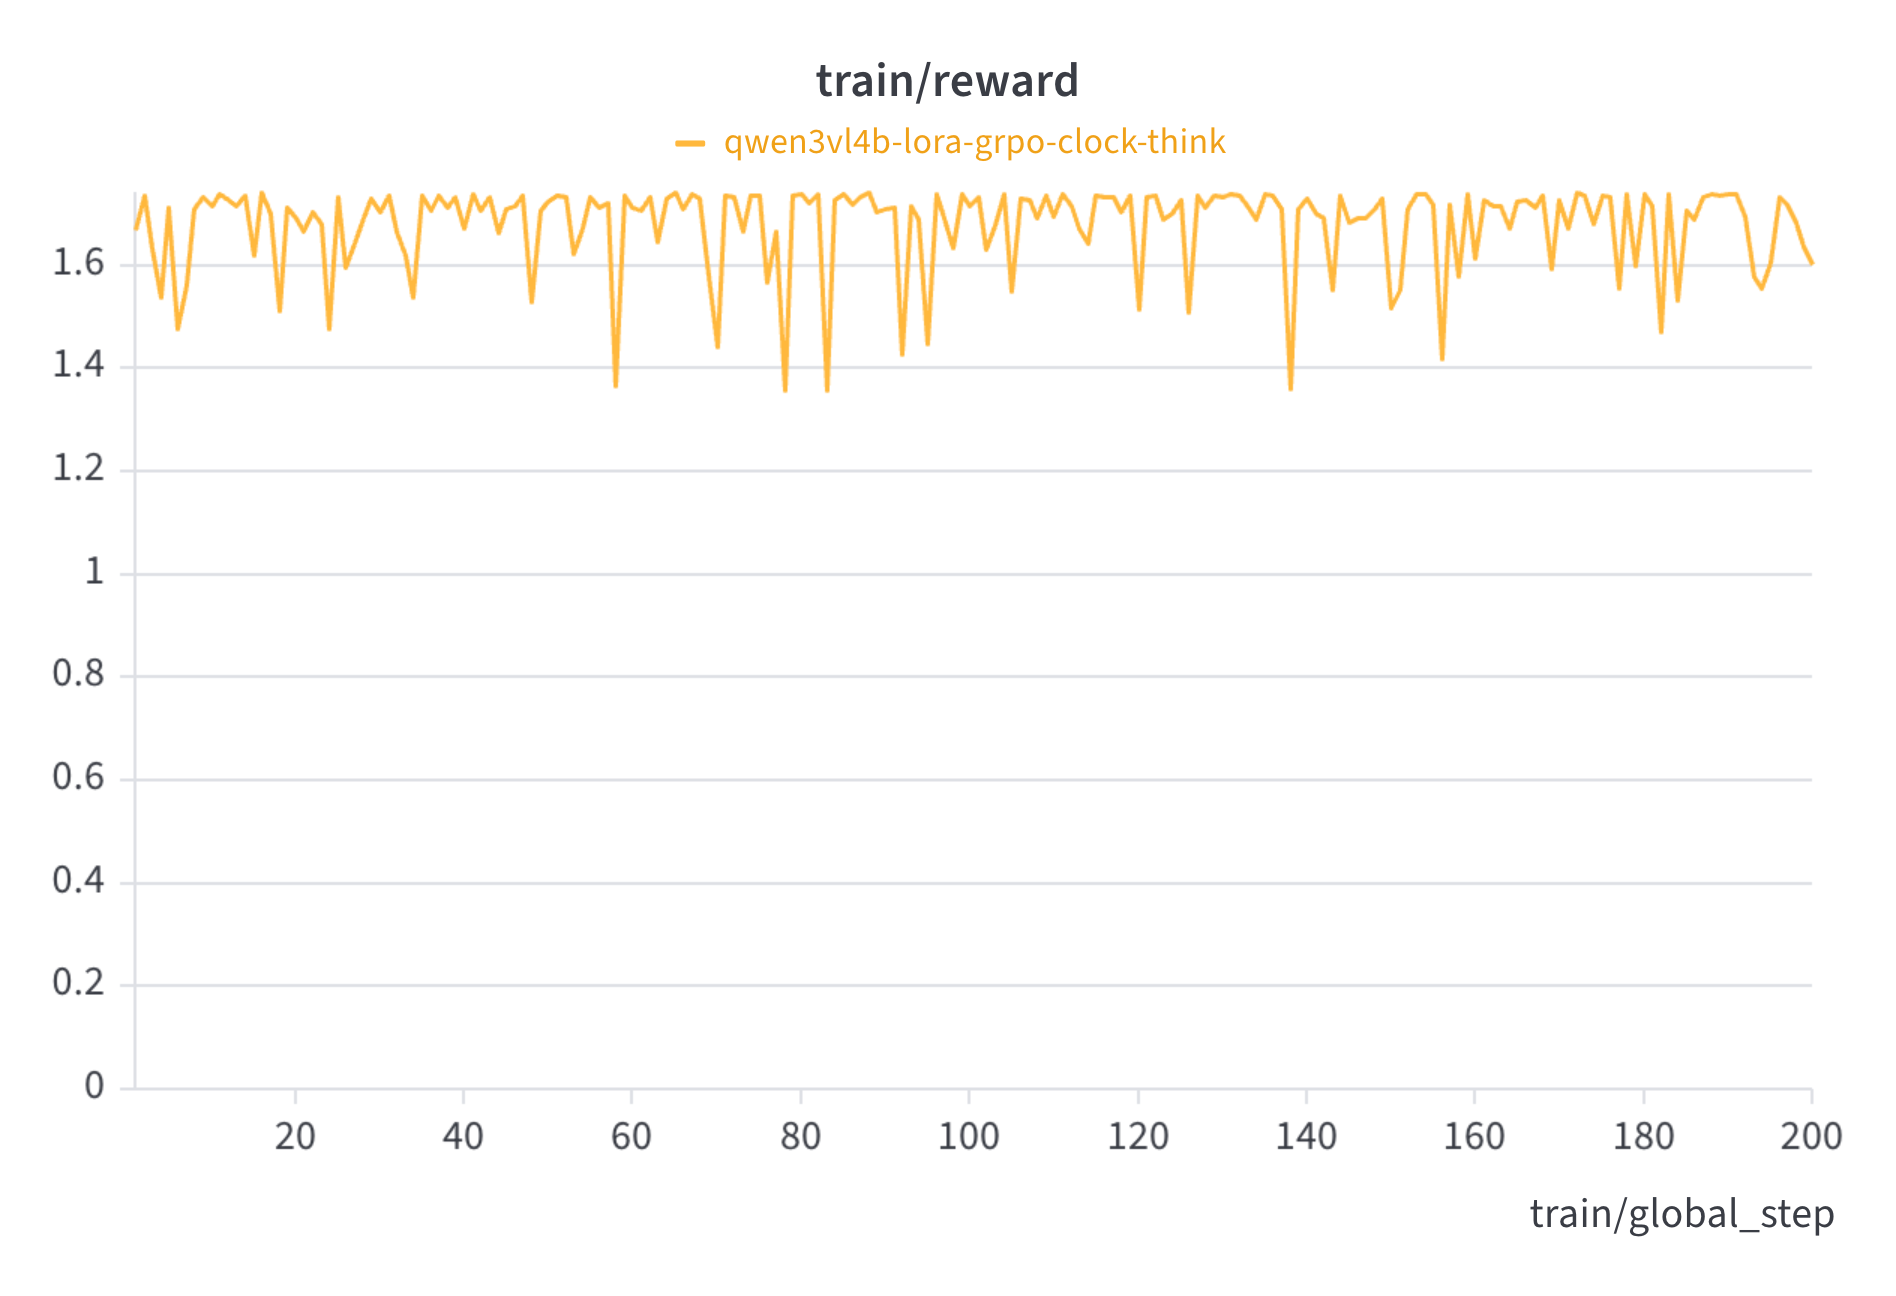
\includegraphics[width=\linewidth]{figs/clock-vlm-grpo-reward.png}
    \small\textbf{Reward}
  \end{minipage}
  \caption{GRPO training curves.}
  \label{fig:grpo-training-curves}
\end{figure}


Here are the results:
% Requires \usepackage{booktabs}
\begin{table}[t]
  \centering
  \caption{Analog clock reading results on the TickTockVQA evaluation set (5,247 images).
  Accuracies are in \%. Minute accuracy allows an error of $\pm$2 minutes. MAE is in minutes.
  $^\dagger$Results reported in the original paper.}
  \label{tab:clock_results}
  \small
  \begin{tabular}{lcccc}
    \toprule
    Model & Hour Acc $\uparrow$ & Minute Acc $\uparrow$ & Full-time Acc $\uparrow$ & MAE (min) $\downarrow$ \\
    \midrule
    \multicolumn{5}{l}{\textit{Zero-shot}} \\
    It's About Time~\cite{itsabouttime}$^\dagger$ & 28.95 & 25.00 & 18.54 & 135.15 \\
    Qwen3-VL-4B (ours, base) & 29.08 & 32.36 & 13.57 & 121.35 \\
    \midrule
    \multicolumn{5}{l}{\textit{Fine-tuned}} \\
    Qwen2.5-VL-7B w/ Swap-DPO$^\dagger$ & 35.39 & 46.16 & 23.06 & 96.42 \\
    Qwen3-VL-4B + SFT (ours) & 51.32 & 51.44 & 36.38 & 78.60 \\
    Qwen3-VL-4B + SFT + GRPO (ours) & 51.44 & 50.70 & 35.66 & 76.91 \\
    \bottomrule
  \end{tabular}
\end{table}

\section{Effects of GRPO and reasoning process}
As shown in ~\autoref{tab:clock_results}, while the accuracy of applying GRPO was comparable to that of SFT, all outputs conformed to the template format. I picked up some images and how its reasoning is changing.
% ---------------- qualitative examples ----------------
% Each row is the same image answered by a different checkpoint (same prompt, greedy decoding).
% Consecutive GRPO checkpoints with identical reasoning are merged into one row.
% Prediction colour: green = within 5 min, amber = within 30 min, red = further off.
% \stated{...} marks the conclusion stated in the reasoning; \tick{...} marks the minute reading in ticks.

% ---- clock_052.jpg ----
\begin{figure*}[p]
  \centering
  \begin{minipage}[t]{0.25\textwidth}
    \vspace{0pt}
    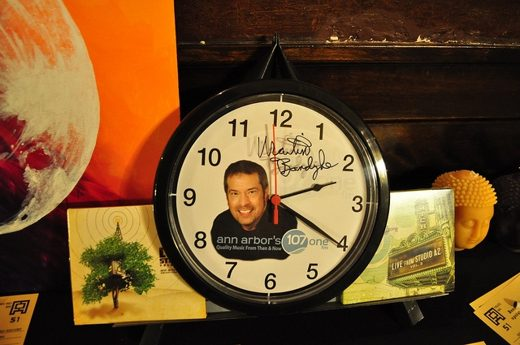
\includegraphics[width=\linewidth]{figs/clock_052.jpg}\\[2pt]
    {\small\textbf{GT 2:20}}\\
    {\scriptsize clock\_052.jpg · COCO 2017 · CC BY 4.0}
  \end{minipage}\hfill
  \begin{minipage}[t]{0.72\textwidth}
    \vspace{0pt}
    \footnotesize
    \begin{tabularx}{\linewidth}{@{}l l l >{\raggedright\arraybackslash}X@{}}
    \toprule
    Checkpoint & Pred. & Error & Reasoning \\
    \midrule
    Base & \errmiss{4:20} & 120 min off & On the clock face, the shorter hour hand is just past the 4, and the longer minute hand is pointing at the 4, which represents 20 minutes. The hour hand being just past 4 confirms it's 4:20. \\
    SFT & \errmiss{12:14} & 126 min off & Locating the clock face. The hour hand (shorter) is about a quarter of the way from the 12 to the 1. The minute hand (longer) \tick{is 4 ticks past the 2}, so 10 + 4 = 14 minutes. At 14 minutes the hour hand should be 23\% of the way past the 12, which matches. \stated{The time is 12:14.} \\
    GRPO step 50--200 & \errok{2:21} & exact & There is one analog clock. The hour hand (shorter) is about a quarter of the way from the 2 to the 3. The minute hand (longer) \tick{is 1 tick past the 4}, so 20 + 1 = 21 minutes. At 21 minutes the hour hand should be 35\% of the way past the 2, which matches. \stated{The time is 2:21.} \\
    \bottomrule
    \end{tabularx}
  \end{minipage}
  \caption{\textbf{Hour fixed early.} SFT puts the hour hand near the 12 (12:14). By GRPO step 50 it reads the hour hand between the 2 and the 3 and the minute hand 1 tick past the 4: 2:21, one minute off. The answer then stays fixed.}
  \label{fig:clock_052}
\end{figure*}

% ---- clock_088.jpg ----
\begin{figure*}[p]
  \centering
  \begin{minipage}[t]{0.25\textwidth}
    \vspace{0pt}
    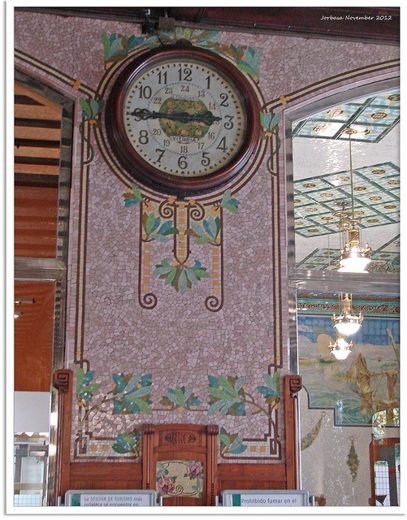
\includegraphics[width=\linewidth]{figs/clock_088.jpg}\\[2pt]
    {\small\textbf{GT 3:15}}\\
    {\scriptsize clock\_088.jpg · COCO 2017 · CC BY 4.0}
  \end{minipage}\hfill
  \begin{minipage}[t]{0.72\textwidth}
    \vspace{0pt}
    \footnotesize
    \begin{tabularx}{\linewidth}{@{}l l l >{\raggedright\arraybackslash}X@{}}
    \toprule
    Checkpoint & Pred. & Error & Reasoning \\
    \midrule
    Base & \errmiss{10:20} & 295 min off & The analog clock shows the hour hand pointing just past the 10 and the minute hand pointing at the 4, which indicates 10:20. \\
    SFT & \errnear{2:46} & 29 min off & Locating the clock face. The hour hand (shorter) is about three quarters of the way from the 2 to the 3. The minute hand (longer) \tick{is 1 tick past the 9}, so 45 + 1 = 46 minutes. At 46 minutes the hour hand should be close to the 3 without reaching it, which matches, so the hour is still 2. \stated{The time is 2:46.} \\
    GRPO step 50 & \errnear{2:46} & 29 min off & There is one analog clock. The hour hand (shorter) is about three quarters of the way from the 2 to the 3. The minute hand (longer) \tick{is 1 tick past the 9}, so 45 + 1 = 46 minutes. At 46 minutes the hour hand should be close to the 3 without reaching it, which matches, so the hour is still 2. \stated{The time is 2:46.} \\
    GRPO step 100--200 & \errok{3:16} & exact & There is one analog clock. The hour hand (shorter) is about a quarter of the way from the 3 to the 4. The minute hand (longer) \tick{is 1 tick past the 3}, so 15 + 1 = 16 minutes. At 16 minutes the hour hand should be 27\% of the way past the 3, which matches. \stated{The time is 3:16.} \\
    \bottomrule
    \end{tabularx}
  \end{minipage}
  \caption{\textbf{Hand confusion fixed by step 100.} SFT reads 2:46: it treats the hour hand as past the 9 position and puts the hour before the 3. From step 100 the model reads the minute hand at the 3 and the hour hand just past the 3: 3:16.}
  \label{fig:clock_088}
\end{figure*}

% ---- clock_037.jpg ----
\begin{figure*}[p]
  \centering
  \begin{minipage}[t]{0.25\textwidth}
    \vspace{0pt}
    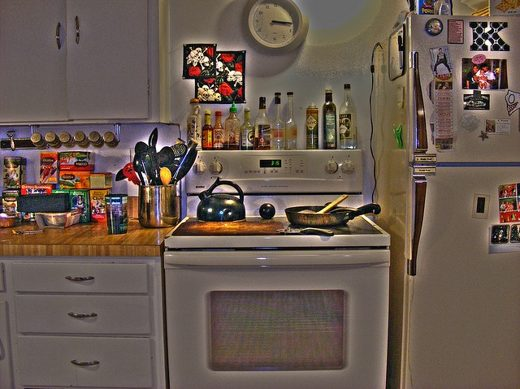
\includegraphics[width=\linewidth]{figs/clock_037.jpg}\\[2pt]
    {\small\textbf{GT 3:15}}\\
    {\scriptsize clock\_037.jpg · COCO 2017 · CC BY 4.0}
  \end{minipage}\hfill
  \begin{minipage}[t]{0.72\textwidth}
    \vspace{0pt}
    \footnotesize
    \begin{tabularx}{\linewidth}{@{}l l l >{\raggedright\arraybackslash}X@{}}
    \toprule
    Checkpoint & Pred. & Error & Reasoning \\
    \midrule
    Base & \errnear{3:40} & 25 min off & The analog clock has its hour hand pointing just past the 3 and its minute hand pointing at the 8, which indicates 3:40. \\
    SFT & \errmiss{12:17} & 178 min off & There is one analog clock. The hour hand (shorter) is about a quarter of the way from the 12 to the 1. The minute hand (longer) \tick{is 2 ticks past the 3}, so 15 + 2 = 17 minutes. At 17 minutes the hour hand should be 28\% of the way past the 12, which matches. \stated{The time is 12:17.} \\
    GRPO step 50--100 & \errmiss{1:16} & 119 min off & There is one analog clock. The hour hand (shorter) is about a quarter of the way from the 1 to the 2. The minute hand (longer) \tick{is 1 tick past the 3}, so 15 + 1 = 16 minutes. At 16 minutes the hour hand should be 27\% of the way past the 1, which matches. \stated{The time is 1:16.} \\
    GRPO step 150--200 & \errok{3:11} & 4 min off & There is one analog clock. The hour hand (shorter) is about a quarter of the way from the 3 to the 4. The minute hand (longer) \tick{is 1 tick past the 2}, so 10 + 1 = 11 minutes. At 11 minutes the hour hand should be 18\% of the way past the 3, which matches. \stated{The time is 3:11.} \\
    \bottomrule
    \end{tabularx}
  \end{minipage}
  \caption{\textbf{Fixed late, in two moves.} SFT reads 12:17. Step 50 moves the hour to 1 (1:16). Only at step 150 does the hour reach 3: 3:11, 4 minutes off. The minute reading stays ``1 tick past'' a mark throughout.}
  \label{fig:clock_037}
\end{figure*}

% ---- clock_081.jpg ----
\begin{figure*}[p]
  \centering
  \begin{minipage}[t]{0.25\textwidth}
    \vspace{0pt}
    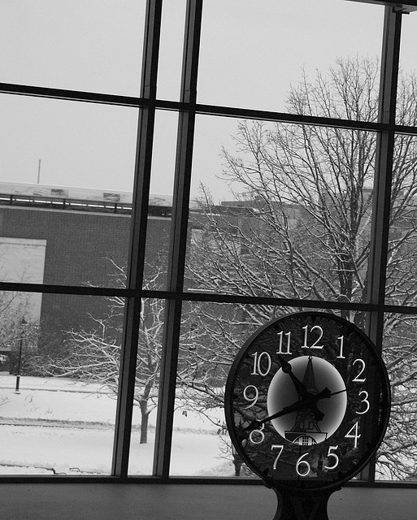
\includegraphics[width=\linewidth]{figs/clock_081.jpg}\\[2pt]
    {\small\textbf{GT 10:41}}\\
    {\scriptsize clock\_081.jpg · COCO 2017 · CC BY 4.0}
  \end{minipage}\hfill
  \begin{minipage}[t]{0.72\textwidth}
    \vspace{0pt}
    \footnotesize
    \begin{tabularx}{\linewidth}{@{}l l l >{\raggedright\arraybackslash}X@{}}
    \toprule
    Checkpoint & Pred. & Error & Reasoning \\
    \midrule
    Base & \errok{10:40} & exact & Hour hand is between 10 and 11, closer to 11. Minute hand is on 8, which is 40 minutes. So time is 10:40. \\
    SFT & \errok{10:43} & 2 min off & Locating the clock face. The hour hand (shorter) is about three quarters of the way from the 10 to the 11. The minute hand (longer) \tick{is 3 ticks past the 8}, so 40 + 3 = 43 minutes. At 43 minutes the hour hand should be 72\% of the way past the 10, which matches. \stated{The time is 10:43.} \\
    GRPO step 50 & \errok{10:41} & exact & There is one analog clock. The hour hand (shorter) is about three quarters of the way from the 10 to the 11. The minute hand (longer) \tick{is 1 tick past the 8}, so 40 + 1 = 41 minutes. At 41 minutes the hour hand should be 68\% of the way past the 10, which matches. \stated{The time is 10:41.} \\
    GRPO step 100 & \errmiss{11:41} & 60 min off & There is one analog clock. The hour hand (shorter) is about three quarters of the way from the 11 to the 12. The minute hand (longer) \tick{is 1 tick past the 8}, so 40 + 1 = 41 minutes. At 41 minutes the hour hand should be 68\% of the way past the 11, which matches. \stated{The time is 11:41.} \\
    GRPO step 150 & \errok{10:41} & exact & \textit{Same reasoning as step 50.} \\
    GRPO step 200 & \errmiss{11:41} & 60 min off & \textit{Same reasoning as step 100.} \\
    \bottomrule
    \end{tabularx}
  \end{minipage}
  \caption{\textbf{Flips back and forth.} SFT reads 10:43 and step 50 sharpens it to 10:41. Then the hour alternates: 11:41 at step 100, 10:41 at step 150, 11:41 again at step 200. The hour hand sits near the 11, where small updates tip the reading.}
  \label{fig:clock_081}
\end{figure*}

\section{Conclusion}
We can see that SFT can significantly improve performance compared to the base model. And for GRPO has improve the reasoning ability without compromising performance. However, further performance improvements may be possible with a more detailed design.


\bibliographystyle{plainnat}
\bibliography{refs}

\end{document}
